\subsection{Case Study}
We collaborated with the domain experts to demonstrate the effectiveness of $\DQV$ by analyzing several real world cases which are slower than our exception.

\subsubsection{Identify the hardware bottleneck}
The first case is executed on a cluster with 5 nodes and run around 623 seconds. The execution plan is shown as the Figure~\ref{fig:teaser}(A).

When exploring the execution with $\DQV$, we find that in the progress view, it is obvious Map1(Figure~\ref{fig:teaser}(B1)) significantly run longer than the duration of other vertices. On the other side, the Reducer2, a subsequent vertex of Map1, finished in a very short time after Map1 is finished. Reducer is followed by a sequence of short reduce vertices(shown as Figure~\ref{fig:teaser}(B3)) which are quickly executed after that. 
From this pattern, we guess the bottleneck should be related Map1, several abnormal tasks may lead to the long execution time of Map1. We hover the mouse on it to highlight the associated tasks as blue color in the Distribution View.
In the summary distribution view, we can see there are two task groups which are distributed far away from each other (shown as Figure~\ref{fig:teaser}(C5, C6)). 
By checking the blue-colored tasks on the machine views through cross-view linking, we find the tasks at the left top corner are dispatched on the machine dbg14, dbg16, dbg19 and dbg20. But the tasks on the right bottom corner are only executed on machine dbg18. Moreover, it seems that dbg18 only executes very few tasks in this case. 
We further check the cluster and notice that something wrong with the network of dbg18, thus the tasks assigned to it are delayed and executed very late, leading to the overall long duration of the query execution. In the exploration of summary view, we can find the these tasks of Map1 provides the data to several tasks of Reducer2, shown as the Figure~\ref{fig:teaser}(C1), which also verifies our assumption. 

In addition to Map1, we notice another vertex Map24 also have a very long duration. When we click to mark the tasks of Map24 (these tasks are colored as purple), we find that none of them are executed on dbg18. So we guess dbg18 is not the only reason results in the slow query. At the same time, there is one task run with a very long time (shown as Figure~\ref{fig:teaser}(C2)) on the machine dbg19. Moreover, the dbg19 executes far fewer tasks than the machine dbg14, dbg16 and dbg20, but these tasks tends to have longer duration. By exploring the performance view, we find the CPU usage view of dbg19 has large piece of red color region, indicating the the CPU is more busy than the other machines(shown as Figure~\ref{fig:teaser}(C3)). We further explore the system log and find there are several computing-bounded programs are executed on dbg19 at the same time which takes the computing resource thus making these query tasks very slow.

\begin{figure}[t]
	\centering
	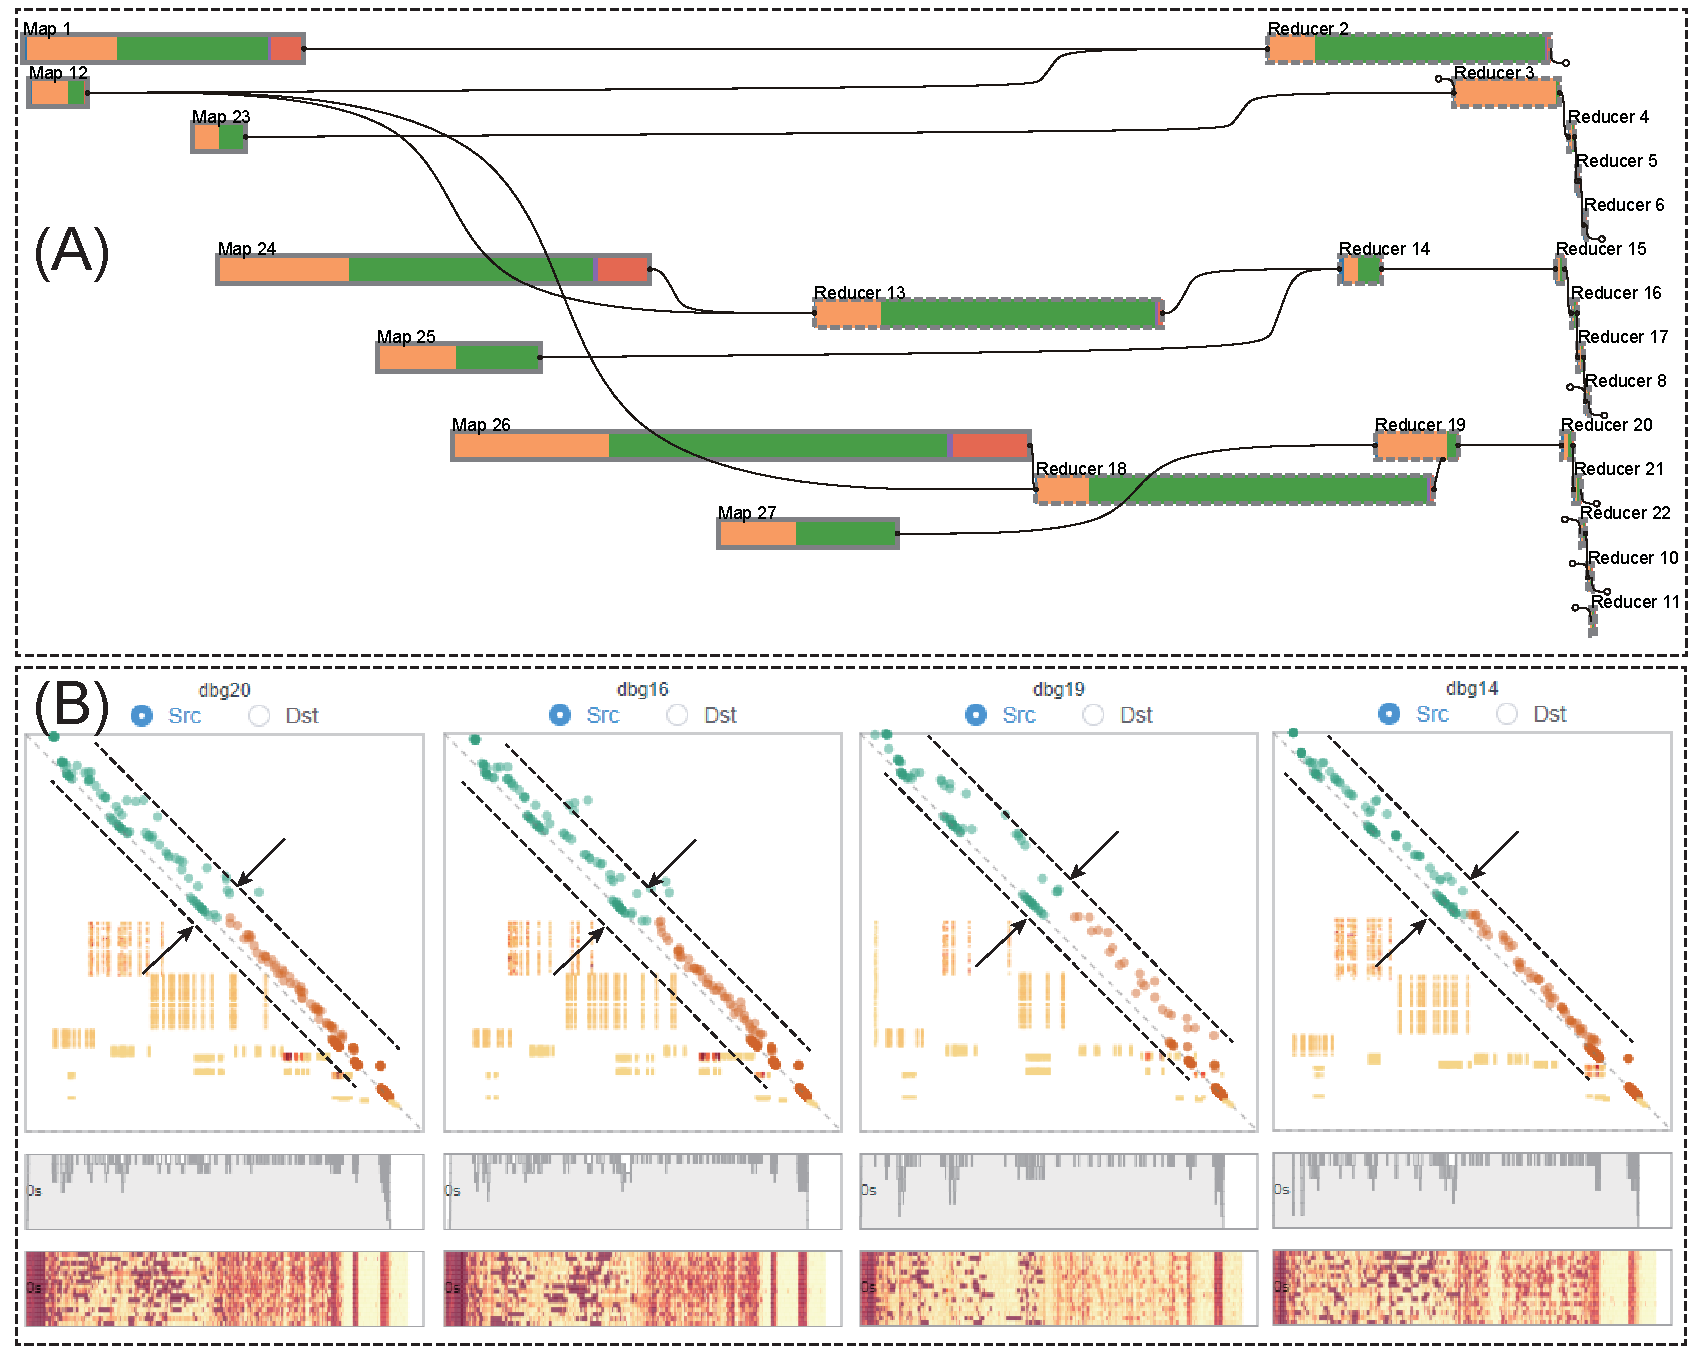
\includegraphics[width=0.48\textwidth]{figures/case_study/CaseStudy1.pdf}
	\vspace{-3mm}
	\caption{Re-execute the query after removing a unhealthy node and stop the CPU-bound programs.}
	\label{fig:casestudy1}
	\vspace{-3mm}
\end{figure}


To address this problem, we directly remove the node dbg18, stop the other programs run on server dbg19 and re-execute the same query. The query is finished with 200s. In the progress view, we find the duration of both vertex Map1 and Map24 are greatly reduced shown as Figure~\ref{fig:casestudy1}(A). We also find that in the distribution view, all the tasks are distributed close to the diagonal line indicating that they are all executed within the small time range Figure~\ref{fig:casestudy1}(B). Moreover, the CPU performance view shows that all the CPUs on different server have the balanced performance. 

\subsubsection{Diagnose the task failure}



\begin{figure*}
	\vspace{2mm}
	\centering
	\small
	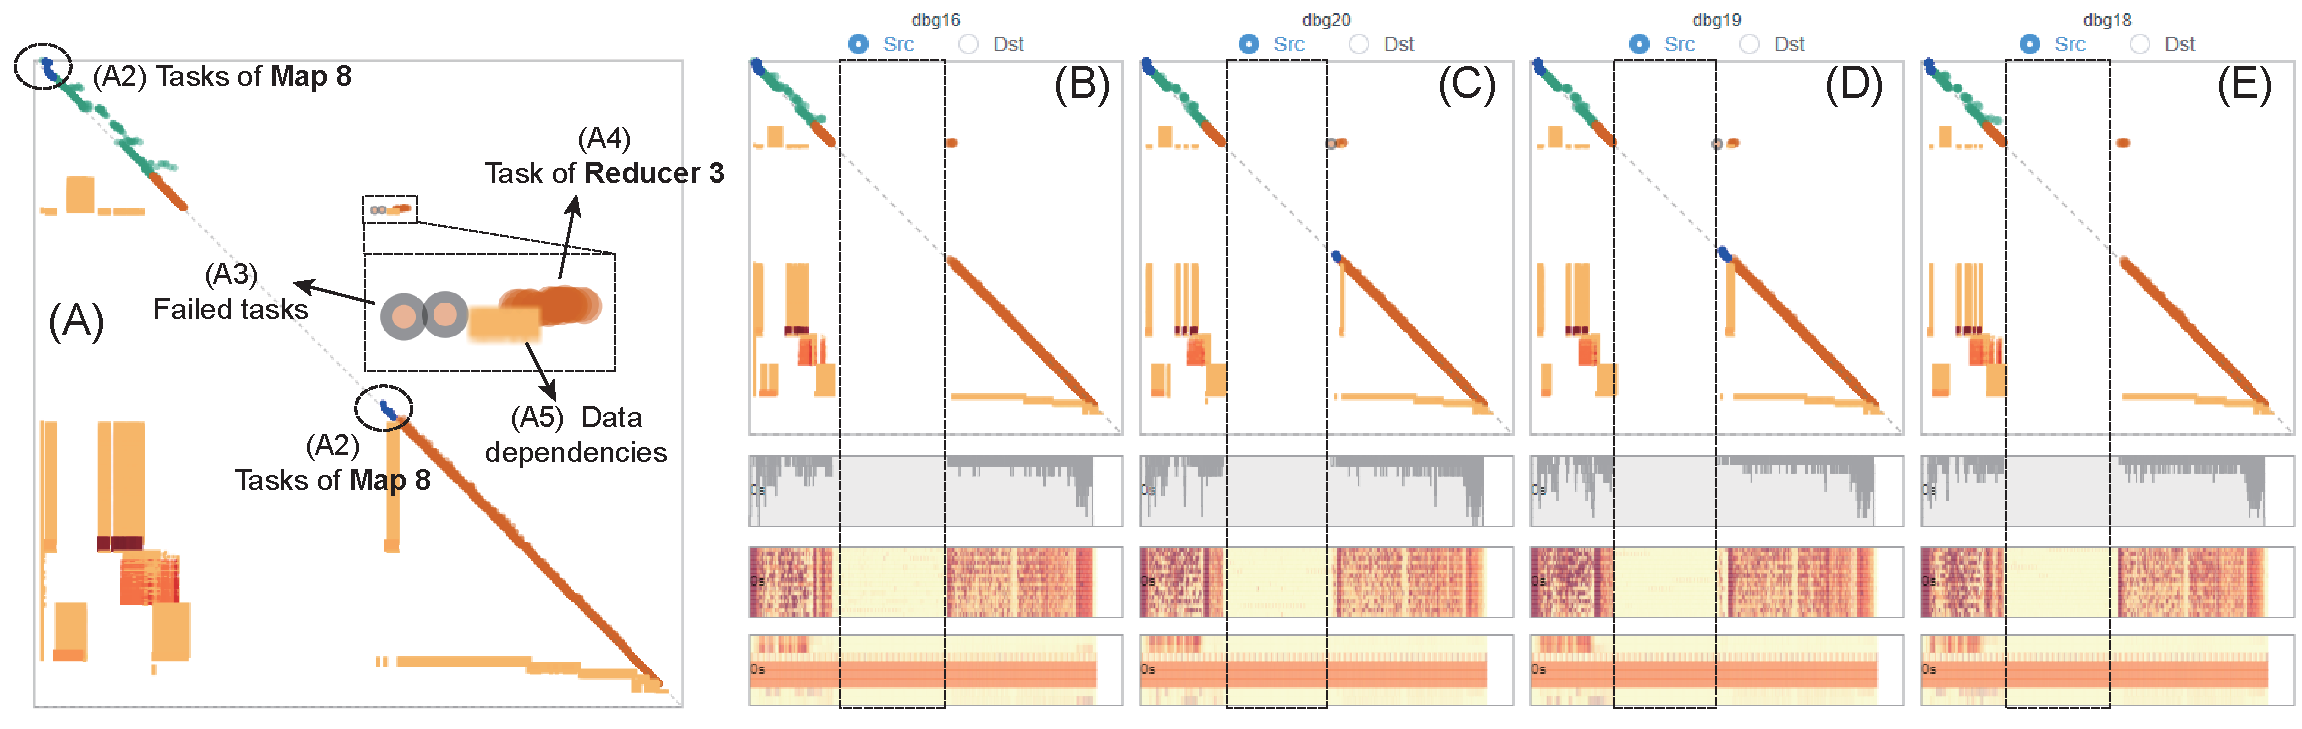
\includegraphics[width=1\textwidth]{figures/case_study/CaseStudy2.pdf}  

	%\vspace{-3mm}
	\caption{Analyze the task failure.} 
	\label{fig:casestudy2}

\end{figure*}


The second case runs on the cluster with four nodes. As shown by the summary view (Figure~\ref{fig:casestudy2}), we find that most of the tasks are located close to the diagonal line, but several reducer tasks associated with Reducer3 have a significant long duration.
Moreover, there are two failed tasks during the execution( Figure~\ref{fig:casestudy2}(A3)). The experts wants to know why these tasks are failed and how the system addresses them. By observing the performance view, we can find that all these four machines execute the maximum number of tasks during the execution of the tasks of Reducer3, shown as the first row in the performance component. 
On the other side, the usage of their CPUs is very low until the failure of the two tasks(shown as the grey stroke circle), which indicates these tasks of Reducer3 use up all the workers but do nothing until the system abandons the two tasks. Moreover, when we highlight the tasks of Map8 by mouse hovering, we find another unusual pattern that the tasks of Map8 form two separated clusters (shown as the blue dots in Figure~\ref{fig:casestudy2}(A1, A2)).  
The tasks shown in Figure~\ref{fig:casestudy2}(A2) are dispatched to the machines dbg20 and dbg19, which just execute the failed tasks(Figure~\ref{fig:casestudy2}(C and D)). Moreover, from the Progress View, we can found that Map8 is one of the preceding vertices of Reducer3. Thus, we infer the failure of these two tasks is caused by the resource deadlock. 

When the system executes the Reducer3 tasks shown in the groupXX, these tasks are waiting for the data from the Map8 tasks shown in Figure~\ref{fig:casestudy2}(A2) as input, but since the Reducer tasks have used all workers in the cluster, the Map8 tasks cannot be scheduled, thus forming the resource deadlock. 
Moreover, the system also has the mechanism to solve this problem: when the system detects long time  of low resource usage, it abandoned two waiting Reduce3 tasks executed on dbg19 and dbg20, free up two workers to execute the Map8 tasks. After that, some of the waiting Reducer3 tasks receive the data and finish quickly. The data dependencies shown as Figure~\ref{fig:casestudy2}(A5) indicates the data transmit from the Map8 tasks shown in Figure~\ref{fig:casestudy2}(A5) to the Reducer3 Tasks shown in Figure~\ref{fig:casestudy2}(A4), which also verify our hypothesis.

\subsubsection{Understand the data skew}

\begin{figure}[t]
	\centering
	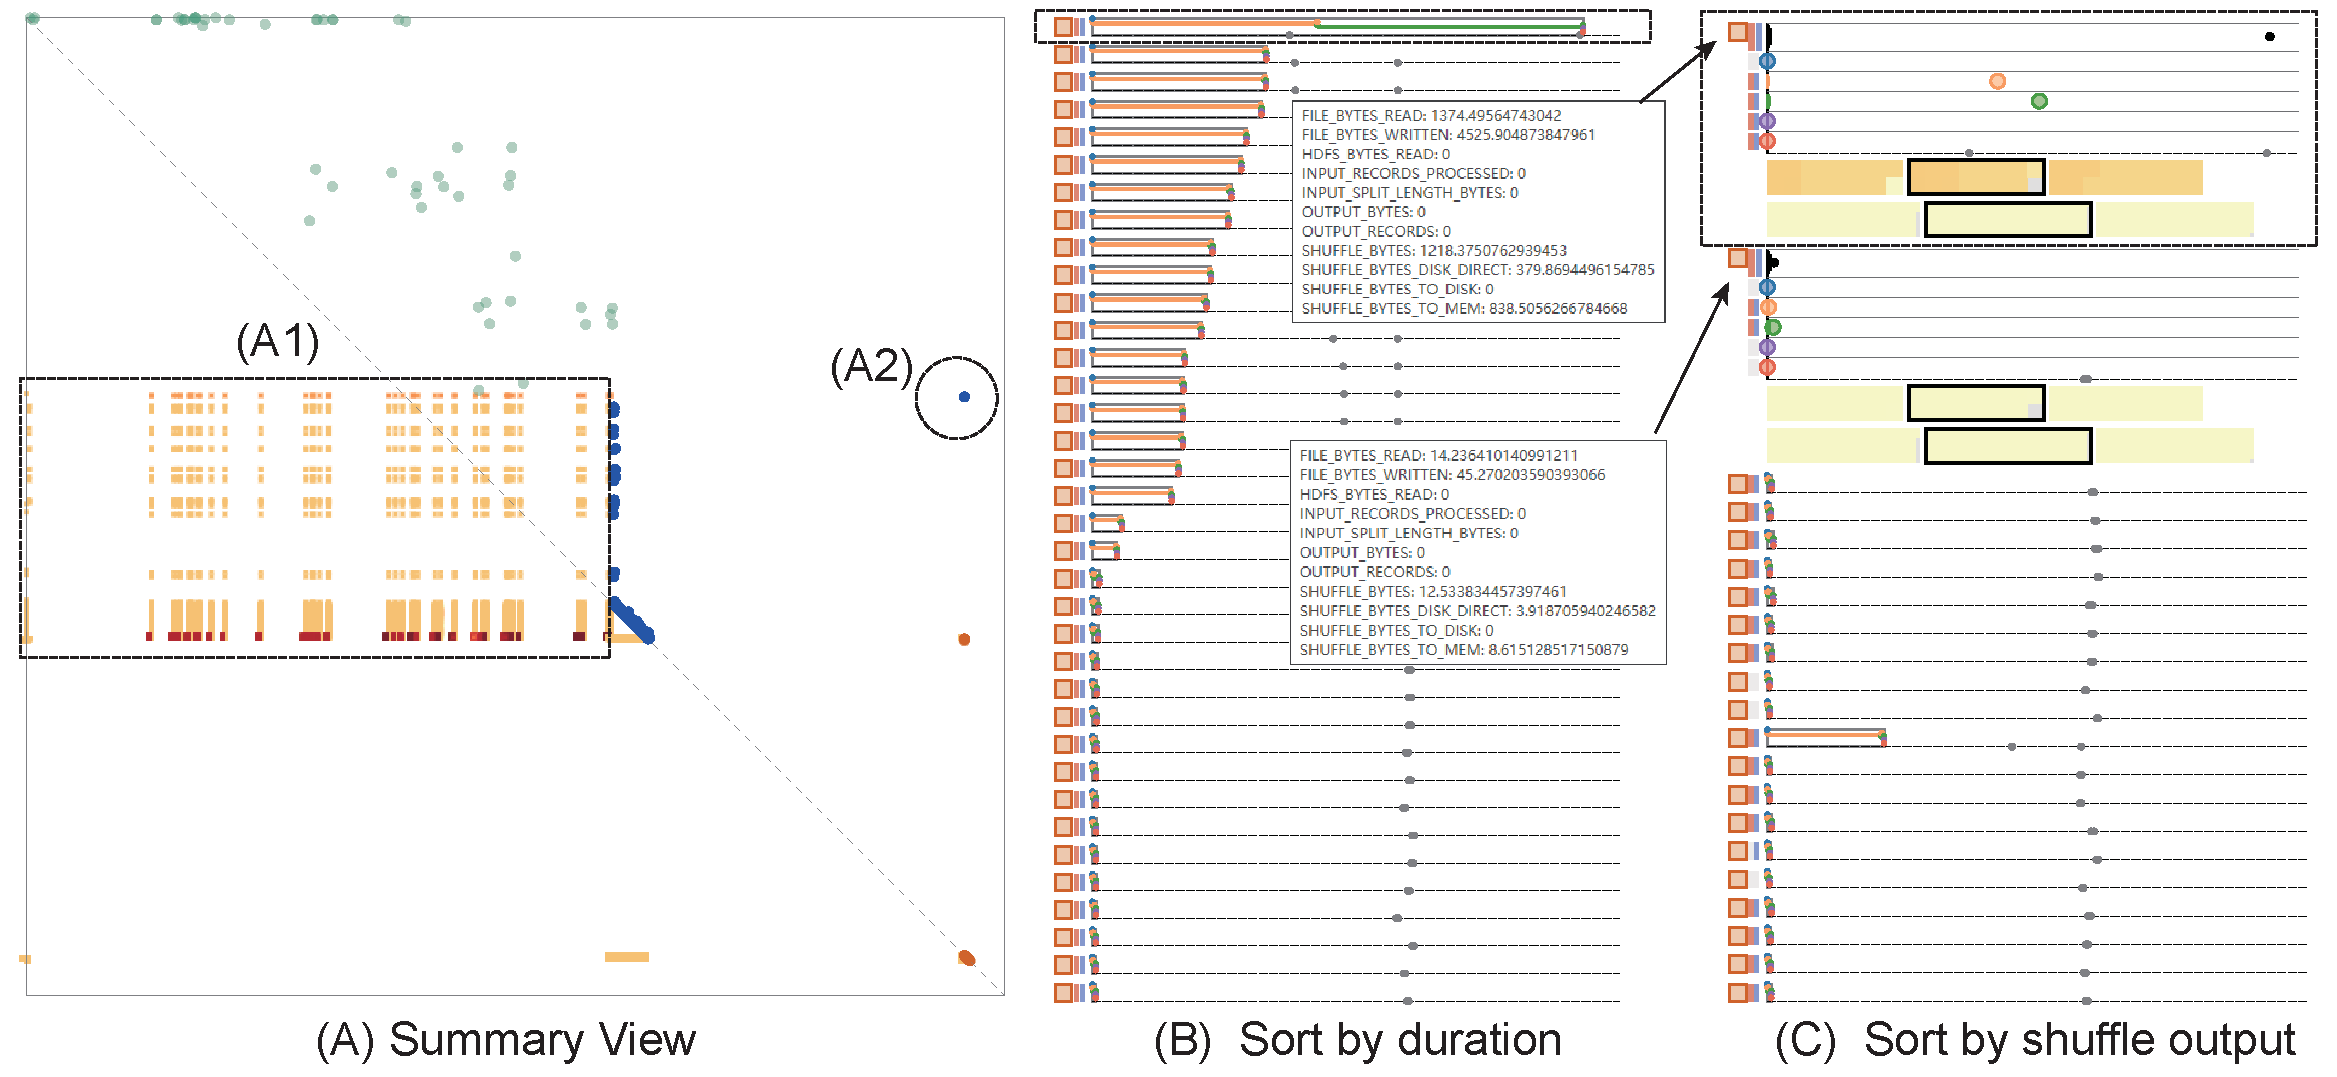
\includegraphics[width=0.5\textwidth]{figures/case_study/CaseStudy3.pdf}
	\vspace{-3mm}
	\caption{Detect the data skew.}
	\label{fig:casestudy3}
	\vspace{-3mm}
\end{figure}

In the third case, we highlight the tasks of Reducer2 by blue color. These tasks can form two groups, the tasks of the first group layout on the vertical line and an outlier point far away from the other points at x-direction, indicating it has a very long duration.
According to the dependencies shown in the region Figure~\ref{fig:casestudy3}(A1), these tasks are waiting for the data from the map tasks shown in region **, and quickly finish once they receive the data. The tasks of the second group layout on the diagonal line, indicating these tasks are quickly finished because they all start after the data is ready. All of the two groups show that the tasks of Reducer2 can be finished quickly. Then, we want to explore why the outlier runs in so slow. We click Reducer2 to list all the tasks in the Task View and sort them by the task duration shown as Figure~\ref{fig:casestudy3}(B). The outlier appears on the top of the task view and has a significant long green bar indicating the processing time, which we guess this task process and generate more data than the other tasks. To verify our assumption, we re-sort these tasks by the input data("FILE BYTES READ") and click the first two tasks to observe their extension form. In the dependency view, we find the source dependency has a dark color than the second task. We further check the amount of data by showing the data information shown as Figure ** and **; we find the input of the first task in 10 more than the second task. These patterns show that this query suffers a serious data skew problem.  

